\chapter{Motivation and theoretical background}

The first section of this chapter lays the theoretical framework of the Standard Model (SM) of particle physics, including the historical discovery timeline of symmetries of nature, each corresponding to a leap forward in our physical understanding, and the model's particle content and their properties. The second section extends the symmetry group of the SM to include candidates for the observed cosmic dark matter (DM) and the particles that could mediate the DM-SM interactions.

\section{The Standard Model}

\subsection{Symmetries of nature}

Each major advance in the history of physics has corresponded to the discovery and mathematical implementation of a new global space-time, global discrete, or local gauge symmetry. In this section, I will review these discoveries, informally developing the mathematical framework needed to understand the symmetry groups of the SM. Along the way, two important subplots will play out: the development of our understanding of physics at smaller distance scales and higher energies, and the unification of previously separate physical sectors.

\indent Our ancient ancestors were aware that certain geometrical shapes, e.g. the Platonic solids, possessed the quality of symmetry, and were driven to understand the composition of physical substances by breaking them down into fundamental, indivisible units. These units, known as atoms by the ancient Greeks, interact and rearrange themselves according to physical laws to account for the variety of substances and physical phenomena we observe. The attraction to applying symmetry to nature is evidenced by the centuries-long belief that the Earth lie at the center of the universe, with the celestial bodies orbiting in perfect, divine circles.

\indent The end of the scientifically repressive middle ages brought along an improvement in astronomical observations and the growth of the pseudo-scientific field of alchemy, which attempted to reduce, understand, and manipulate the fundamental elements of physical substances. When Kepler discovered three laws of planetary motion, he unified the description of the motion of the planets. For the first time, the conservation of a physical quantity, what we now know as angular momentum, was associated with a general set of physical objects. At the burgeoning of the scientific revolution, Newton championed the idea that the same physical laws can be applied to all physical events, and that properties of these laws can be abstracted to apply to nature at a fundamental level.

\indent Newton defined an inertial reference frame implicitly as one where his first law held, that is, that an object remains at constant motion unless acted on by an outside force. Since his laws were the same in all inertial reference frames, a new symmetry of nature was discovered, now called symmetry under Euclidean transformations. Since Euclidean transformations form a mathematical group, it is said that classical mechanics is invariant under the Euclidean group. The invariance under the Euclidean transformations can be used to derive conservation laws: Newton's laws don't depend on spatial translations or rotations, implying the conservation of linear and angular momentum, respectively. These relationships foreshadow Noether's abstraction of the connection between continuous symmetries and conserved quantities. She proved that there is a conserved quantity, or current, associated with every symmetry of a physical system \cite{Noether:1918zz}. This famous theorem facilitates the derivation of conserved quantities and will be used extensively in the theories that follow. The extension of the Euclidean transformations to include time translations and motion at constant velocity (boosts) forms the Galilean group.

\indent The next symmetry of nature to be discovered came when Lorentz found that \\
Maxwell's equations, which unified the classical eletricity and magnetism sectors \cite{Maxwell01011865}, were invariant under a set of transformations that generalized the classical Galiliean translations, now called Lorentz transformations, which form the Lorentz group \cite{Lorentz}. The Lorentz symmetry corresponds to the conservation law of total electric charge \cite{Noether:1918zz2}. Soon after, Einstein derived the Lorentz symmetry as a property of space-time itself through his special theory of relativity, assuming two simple postulates: the laws of physics and the speed of light are the same in all inertial reference frames \cite{Einstein:1905ve}. From these simple assumptions, Einstein was able to extend the classical laws of physics to the high velocity, high energy sector. Before Einstein, the symmetries of nature were thought to be consequences of the physical laws themselves, but Einstein's major paradigm shift was to view the symmetry itself as the more fundamental property, an insight key to his formulation of the general theory of relativity for the gravitational interaction \cite{Einstein:1914bt}, which is not discussed further in this thesis. Combining the Lorentz and Euclidean transformations yields the Poincare group, the final global space-time symmetry of the SM.

\indent Just as relativists were probing physics at higher speeds and energies, other physicists were investigating the behavior of systems at smaller distance scales, conducting experiments to explore phenomena such as the Compton effect \cite{PhysRev.21.483} and photoelectric effect\cite{Einstein:1905cc}, which showed the quantized, particle-like behavior of light, and electron beam diffraction \cite{Davisson:1927ta}, which showed the wave-like behavior of electrons. Quantum theory was developed to consolidate the wave-like and particle-like behaviors of systems, and extended the validity of classical physics to microscopic scales. Where in classical physics particles states were described by their absolute position and momentum, quantum theory describes the state of a system by a probabalistic wavefunction. The classical symmetries and conservation laws carried over to quantum theory, with the concept of angular momentum generalized to include spin. Particles with zero or integer spin are called Bosons, and were shown to obey Bose-Einstein statistics, where the wavefunction is symmetric under all permutations of particles. Particles with half-integer spin, called Fermions, obey Fermi-Dirac statistics, where the wavefunction is symmetric under even permutations and changes sign under odd permutations, implying that no two particles can occupy the same state. These many-particle symmetries were applied to derive properties of materials and states of electrons in atomic and periodic systems, blackbody radiation, and many other properties of matter and radiation \cite{Shankar}.

\indent Quantum theory was successfully applied to a myriad of low-energy systems. Dirac extended quantum theory and the Schrodinger equation, which describes the evolution of a quantum system in time, to the relativistic regime \cite{Diracqm}. His formulation of the wave equation for a spin-1/2 particle with mass m is inherently Lorentz invariant:

\begin{equation}
(i \gamma^\mu \partial_\mu - m)\psi = 0
\end{equation}

\begin{equation}
\frac{dN}{dt} = \sigma\  \mathcal{B}\ \ \ \times\ \ \ L\ \ \ \times\ \ \ \epsilon\ \ \ \times\ \ \ A
\end{equation}

The solutions to the Dirac equation were found to have both positive and negative energy solutions, to the surprise of Dirac. His explanation was that the vacuum consisted of a "sea" of negative energy solutions, each in a distinct state due to the Pauli exclusion principle, and when a pair of electrons was produced, a positive energy state was filled and a negative energy state was vacated, creating a "hole" in the sea. The particle corresponding to this hole would have the same energy as the electron, but in order to conserve total charge, must have the opposite sign charge. This positively charged electron was not know to exist at the time, but was soon discovered in cosmic ray experiments and named the positron \cite{PhysRev.43.491}. Dirac's theoretical prediction of the positron and its subsequent discovery opened the door for the discovery that every particle has an oppositely charged antimatter partner. 

\indent In an attempt to apply relativistic quantum theory to the electromagnetic field and the spin-0 photon, Dirac formulated the theory of quantum electrodynamics (QED) \cite{Dirac243}. QED is the first example of a quantum field theory (QFT), where the physical dynamics apply to the quantum field associated with a particle rather than the particle itself, and particles/antiparticles interact as excitations of the field. This formulation of creation and annihilation of particles and antiparticles gave a more physically intuitive explanation for the negative energy solutions of the Dirac equation than the Dirac sea. QED became the prototype for developing future relativistic quantum theories and Dirac's procedure the template for quantizing a general field theory. 

\indent With the discovery of antimatter and the apparatus of QFT in place, physicists continued searching for additional symmetries. If a particle state is an eigenvector of a symmetry operator, then the eigenvalue is an important quantum number of the state, since if the symmetry is conserved, the quantum number can be used to determine if a decay or interaction of this state is allowed. Three important discrete symmetries operations, and their products, have had significant importance: space coordinate parity inversion (P), particle-antiparticle charge conjugation (C), and time reveral (T) \cite{Bettini}. Violation of P was observed for the weak interactions by Wu and others in the decays of Co-60 atoms \cite{PhysRev.105.1413}. Although it was long believed to be a symmetry of all the interactions, CP, the product of C and P was also found to be violated by the weak decays of K mesons \cite{PhysRevLett.13.138}. It is only the combination of P, C, and T that is now thought to be an exact symmetry of nature, obeyed by all interactions. The CPT symmetry was proven to be conserved in all relativistic QFTs \cite{PhysRev.82.914, Luders:1954zz}.

\indent The mid-20th century saw an explosion of discovery in particle physics and was a golden age for the feedback between theoretical and experimental work. The discovery of additional particles such as the muon \cite{PhysRev.50.263}, pion \cite{Lattes:1947mx}, neutrino\cite{1956Sci...124..103C}, and many others inspired the theoretical development of the quark model \cite{GellMann:1964nj}, the refinement of QED \cite{PhysRev.73.416, PhysRev.74.1439, PhysRev.76.749, PhysRev.76.769, PhysRev.80.440, Tomonaga:1946zz, PhysRev.75.486, PhysRev.75.1736}, and the formulation of theories to explain the strong \cite{GellMann:1964nj, Zweig:1981pd, Zweig:1964jf, PhysRevLett.30.1346, PhysRevD.8.3633} and weak \cite{Fermi:1933jpa} nuclear forces. Conversely, these new theories led to the prediction and subsequent discovery of new fundamental particles, such as the charm \cite{PhysRevLett.33.1406, PhysRevLett.33.1404} and bottom \cite{PhysRevLett.39.252} quarks, and composite particles, such as the $\Omega^-$ \cite{Barnes:1964pd}.

\indent The development of the theories of the strong and weak forces unveiled a new set of symmetries: local invariance under unitary gauge transformations. In keeping with the trend of the discovery of new symmetries being associated with the unification of physical sectors, the electromagnetic and weak nuclear interactions were found to be components of a single force, called the electroweak force \cite{Glashow:1961tr, PhysRevLett.19.1264}. Again, with QED as the prototype, the Langrangians for the electroweak and strong forces were constructed to be invariant under unitary groups. Early work by Weyl \cite{Weyl:1927vd} showing the gauge invariance of electromagnetism was extended to QED, and lay the mathematical framework for describing the gauge invariance of the other forces. To demonstrate gauge invariance and how the gauge group generators are asssociated with the force carriers, take the QED terms of the SM Lagrangian as an example case \cite{peskinschroeder}:

\begin{equation}
\mathcal{L} \supset \bar{\psi} ( i \gamma^\mu D_\mu - m ) \psi - \frac{1}{4} F^{\mu\nu}F_{\mu\nu}
\end{equation}
where $A_\mu$ is the EM 4-potential and field corresponding to the photon, $F^{\mu\nu} = \partial^\mu A ^\nu - \partial^\nu A^\mu$ is the electromagnetic field tensor, and $D_\mu = \partial_\mu + i e A_\mu$ is the gauge covariant derivative. These terms are invariant under the the U(1) transformations

\begin{equation}
\psi \rightarrow e^{i\theta(x)} \psi.
\end{equation}

In general, the generators of an interaction's continuous symmetry group correspond to the gauge fields whose excitations are the gauge bosons that mediate that interaction. Just how $A_\mu$ is the field corresponding to the photon in QED and generator of the U(1) symmetry group of EM, the W and Z bosons and gluons are formed from the generators of the symmetry groups for the electroweak and strong interactions, SU(2)xU(1) and SU(3), respectively. Additionally, the covariant derivative is transformed in a way analagous to the QED covariant derivative, adding a factor for each generator with the corresponding charge in the coefficient. These charges (electric, color, weak isospin and hypercharge) are conserved for all of the forces in all interactions\cite{Bettini}. The charges of the SM particles are described in more detail in the next section.

\indent Although the mathematical descriptions of their symmetries are similar, the EM, weak, and strong nuclear forces are quite different qualitatively. The EM force is the most familiar, being responsible for the interactions of matter and radiation at macroscopic scales, having only one type of charge which can be postitive or negative. The strong force is mediated by eight gluons, corresponding to the eight generators of SU(3), and carries three types of charge, known as red($R$), green($G$), and blue($B$). The "negatives" of these charges are called anticolors: antired($\bar{R}$), antigreen($\bar{G}$), and antiblue($\bar{B}$). Keeping with the visible color analogy, the theory of the strong force is called quantum chromodynamics (QCD). At low energies, the quarks and antiquarks are confined to form only color-neutral states. This is known as color confinement, and implies no free quarks exist, but only come in neutral combinations called hadrons. Since hadrons are strictly color-neutral, their states transform as the singlet representation under SU(3). At high energies, the strong coupling decreases, and the quarks can be treated as effectively free particles with perturbation theory using Feynman diagrams. This property of the strong force is known as asymptotic freedom. The weak force is qualitatively different than either the EM or strong forces, as particles do not exchange its mediators to form bound states of any kind. The low-energy limit of the weak theory was developed by Fermi to explain beta decays \cite{Fermi:1933jpa}, but the full description was not developed until the electroweak force was formulated. 

\indent The unification of the electromagnetic and weak interactions into the electroweak force at about 100 GeV had one major shortcoming: the invariance of the Lagrangian required the gauge bosons, $B$ from U(1) and $W^1, W^2, W^3$ from SU(2), to be massless. While the photon is indeed massless, the W and Z bosons have a nonzero mass \cite{}. Higgs and others \cite{PhysRevLett.13.321, Higgs:1964ia, PhysRevLett.13.508, PhysRevLett.13.585, PhysRev.145.1156, Kibble:1967sv} proposed a solution by introducing a new scalar field whose excitations were called the Higgs boson (H). The scalar field is a complex doublet, meaning it has four total real components, and its vacuum expectation value (vev), or value throughout all of space, is one of many non-zero values in the bottom of its "Mexican hat" potential. This spontaneous symmetry can be broken by choosing one of the values for the vev: $H = \frac{1}{\sqrt{2}} (0, \nu)$, where $\nu=246$ GeV is called the H vev. At energies above $O(100)$ GeV, the electroweak symmetry is obeyed, the gauge bosons are massless, and the Higgs field has one of many values along the circle at the base of its potential. When the H field is expressed as a perturbation about this vev, the electroweak symmetry is broken into the weak and EM forces, and mass terms are generated for the weak force bosons, which are expressed as linear combinations of $B, W^1, W^1, W^3$. The process of the Higgs acquiring a vev, spontaneously breaking the symmetry in its potential, and generating the masses of the weak bosons, is know as the Higgs mechanism, and results in the breaking of the electroweak symmetry. This mechanism can be carried out for a general operator depending on H with the substitution

\begin{equation}
H \rightarrow \frac{1}{\sqrt{2}} (\nu + h)
\end{equation}
where $h$ is the physical Higgs, corresponding to the leftover degree of freedom of the H doublet that is not absorbed by the three massive gauge bosons. H couples to the SM fermions, detailed in the next section, not by the same mixing as described for the gauge bosons, but via Yukawa interactions, direct couplings whose coefficients are related the the fermion masses. The Higgs mechanism was the final piece of the puzzle to understanding the fundamental laws of particle physics.
 
\indent The final result of this saga is the standard model of particle physics, a relativistic gauge quantum field theory, globally invariant under the Poincare group, and locally invariant under the product of the strong and electroweak symmetry groups, which describes all of the fundamental particles and their interactions. The particle content of the SM is detailed in the next section.

\subsection{Particle content}

The particle content of the SM is displayed in Figure~\ref{fig:smparticles}

\begin{figure}[tbh]
\centering
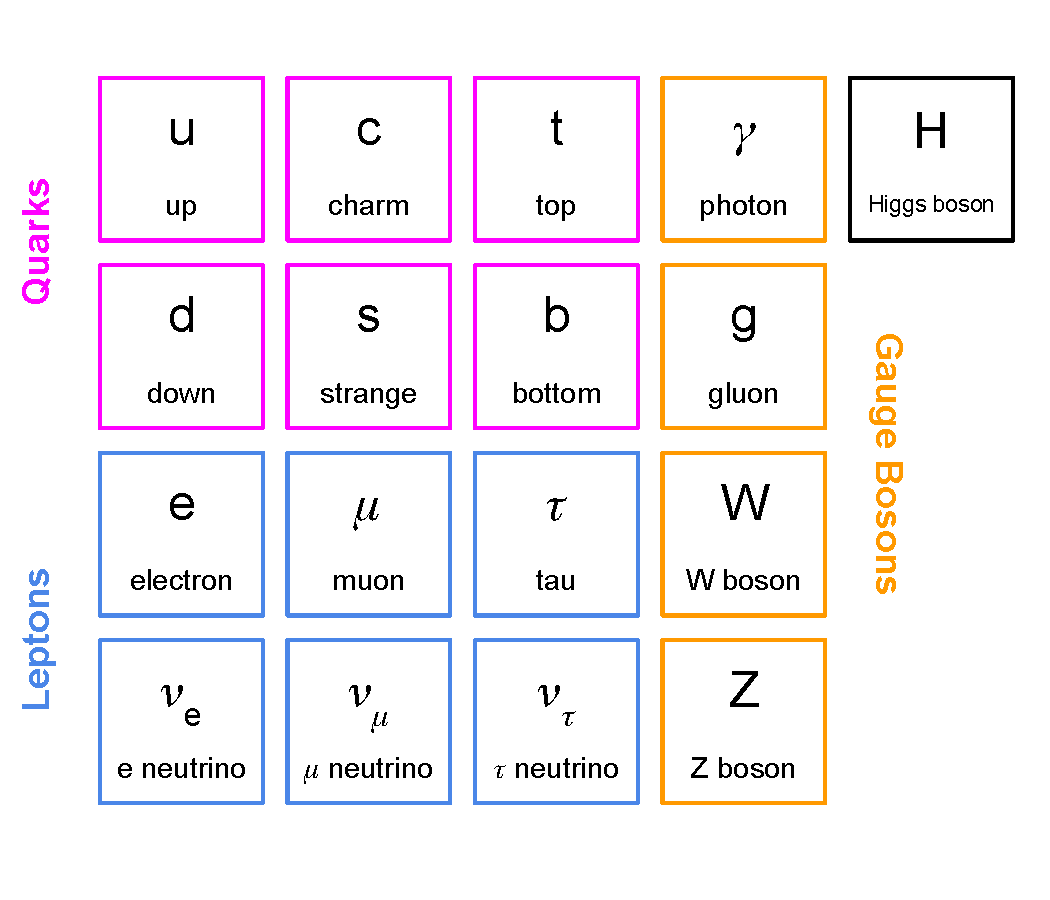
\includegraphics[width=3in]{figures/smparticles.pdf}
\caption{Particles of the Standard Model.}
\label{fig:smparticles}
\end{figure}

The particles of the standard model consist of the spin-1/2 fermions, which interact to form regular matter, the spin-1 bosons, which mediate the interactions of the fermions, and the spin-0 scalar Higgs boson, which generates the masses of the bosons and fermions via the Higgs mechanism. Unless otherwise labeled, the material in this section comes from \cite{Bettini}.

\indent The fermions come in three sets of increasing masses, called generations, corresponding to the first three columns of Table~\ref{tab:sm}. Across the rows, the particles have similar properties, and are abbreviated $u^i, d^i, e^i, \nu_e^i$ from top to bottom with $i=1,2,3$ the generation index. Within each generation, the fermions are divided into two categories: the quarks, which are charged under the EM, weak, and strong forces, and the leptons, which are charged under the EM and weak forces. Each fermion has a corresponding antiparticle, whose mass is the same, but whose charges are opposite in sign. The quarks are SU(3) triplets, having a color charge of either R, G, or B. Since the weak force violates P, the fermions can be distinguished by their chirality, being labelled as either right handed ($e^i_R$) or left handed ($e^i_L$). The $(u^i, d^i)_L$ and $(e^i, \nu_e^i)_L$ pairs and their right handed anti-particle pairs are SU(2) doublets and interact via the weak force. The right handed fermions (left handed anti-fermions) are SU(2) singlets and do not interact via the weak force. The weak isospins ($T_3$) for the left handed fermions are: $(u^i, d^i)_L = (1/2, -1/2)$ and $(e^i, \nu_e^i)_L = (-1/2, 1/2)$. The EM charges are $(u^i, d^i)_L = (2/3e, -1/3e)$ and $(e^i, \nu_e^i)_L = (-1e, 0)$, and finally, the weak hypercharges are, from the relation $Y_W = 2(Q-T_3)$, $(u^i, d^i)_L = (1/3, 1/3)$ and $(e^i, \nu_e^i)_L = (-1, -1)$.

\indent The fourth column of Table~\ref{tab:sm} lists the force mediators, or gauge bosons. g stands for the 8 gluons of QCD that mediate the strong nuclear force. The gluons are octets under SU(3), and correspond to linear combinations of the generator gauge fields $G^a_\mu$. Gluons carry color charge themselves, but are electrically neutral. They are massless, consistent with the fact that they correspond to generators of a conserved symmetry, and may be represented using the Gell-Mann matrices as the linearly independent set of states \cite{Griffithsqm}:

\begin{equation}
\begin{split}
\frac{1}{\sqrt{2}}(r\bar{b} + b\bar{r}) \\
\frac{1}{\sqrt{2}}(r\bar{g} + g\bar{r}) \\
\frac{1}{\sqrt{2}}(b\bar{g} + g\bar{b}) \\
\frac{1}{\sqrt{2}}(r\bar{r} - b\bar{b}) \\
-i \frac{1}{\sqrt{2}}(r\bar{b} - b\bar{r}) \\
-i \frac{1}{\sqrt{2}}(r\bar{g} - g\bar{r}) \\
-i \frac{1}{\sqrt{2}}(b\bar{g} - g\bar{b}) \\
\frac{1}{\sqrt{6}}(r\bar{r} + b\bar{b} -2g\bar{g}),
\end{split}
\end{equation}

while the color singlet state that the colorless hadrons are in is:

\begin{equation}
\frac{1}{\sqrt{3}}(r\bar{r} + g\bar{g} + b\bar{b}).
\end{equation}

\indent The remaining gauge bosons mediate the electroweak force. Before electroweak symmetry breaking, the generators of SU(2)xU(1) correspond to the gauge fields \\
$B,\  W^1,\  W^2,\  W^3$, whose excitations are massless gauge bosons. After symmetry breaking via the Higgs mechanism, three of the bosons acquire mass and the electroweak gauge bosons are reparametrized as:

\begin{equation}
\begin{split}
W^\pm = \frac{1}{\sqrt{2}}(W^1 \pm iW^2) \\
Z = \cos\theta_w W^3 - \sin\theta_w B \\
\gamma = \sin\theta_w W^3 + \cos\theta_w B \\
\end{split}
\end{equation}
where $\theta_w$ is the weak mixing angle, the massive $W^\pm$ and $Z$ bosons mediate the weak force, and the massless $\gamma$ is the photon which mediates EM. $W^\pm$ have electric charge $\pm 1e$ while the $Z$ and $\gamma$ are neutral. The isospin of $W^\pm$ is $\pm1$ and 0 for $Z$ and $\gamma$, giving hypercharges of $0$ for $W^\pm$ and 0 for $Z$ and $\gamma$. 

\indent The final particle of the SM is the scalar H. H is electrically neutral and constructed to be an SU(2) doublet before electroweak symmetry breaking, with one component having weak isospin 1/2 (hypercharge -1), and the neutral component having isospin -1/2 (hypercharge 1), which includes the physical h. After electroweak symmetry breaking, three of the H components are absorbed by the gauge bosons, and the remaining physical h remains neutral. The parity of h is 1. Although H couples to all massive fermions and bosons, the decay channels that are relevant for collider searches are: $ZZ^* \rightarrow 4l,\  WW^* \rightarrow 2l2\nu,\  \gamma\gamma,\  \tau\bar{\tau},$ and $b\bar{b}$. After a decades long search, the discovery and verification of quantum numbers of H was announced by the CMS and ATLAS exeriments in 2012 \cite{Chatrchyan:2012xdj, Aad:2012tfa}. The four-lepton invariant mass distribution, showing the H peak at its observed mass of $m_H = 126$ GeV is shown in Figure~\ref{4l} \cite{CMS:HZZ}.

\begin{figure}[tbh]
\centering
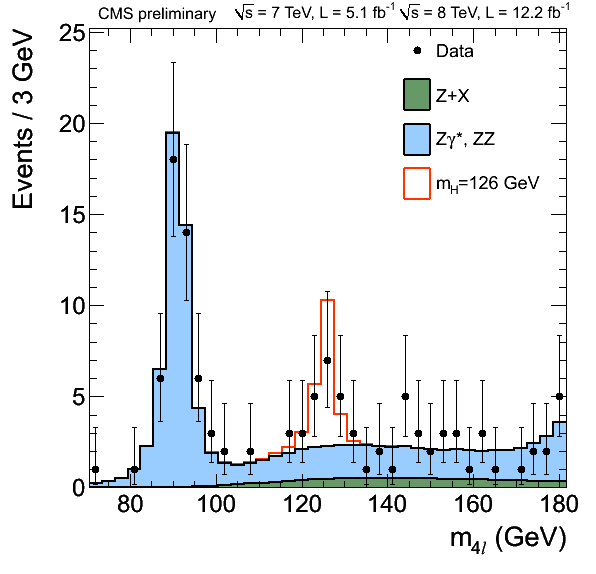
\includegraphics[width=3in]{figures/ZZMass_7Plus8TeV_70-180_3GeV.png}
\caption{4l invariant mass distribution showing H discovery in the ZZ* decay channel. The red line shows the signal distribution for $m_H=126$ GeV.}
\label{4l}
\end{figure}


\section{Dark matter}

\subsection{Background}

This section gives an overview of the most compeling sources of observational evidence for the existance of DM, the potential particles candidates for DM, and the potential methods for detecting them.  

\subsubsection{Observational evidence}

The earliest indication that there may be matter in the universe that cannot be detected by conventional optical observations, so called dark matter (DM), came from measurements of the orbital velocities of astronomical bodies in galaxy clusters \cite{Kapteyn:1922zz, Zwicky:1937zza} and galaxies \cite{Rubin:1970zza, Rubin:1980zd}. Classical Newtonian gravity gives a galactic rotation curve, which shows how the velocity $v$ of a massive object depends on its distance $r$ from the center of a galaxy, as $v(r) \propto \sqrt{M(r)/r}$, where $M(r)$ is the total mass in the galaxy within a radius $r$. However, measurements of the orbital velocities of objects outside of the visible part of galaxies, where $v(r) \propto 1/\sqrt{r}$, show instead $v(r) \propto$ const., i.e. that the mass $M(r) \propto r$ instead of being constant \cite{Agashe:2014kda}. The larger than expected velocities imply the existance of this spherically symmetric, dark halo of non-luminous matter in galaxies. 

\indent A compelling example showing direct evidence for DM is galaxy cluster 1E0657-558, often referred to as the "bullet cluster" from its bullet-like shape \cite{Clowe:2003tk}. The bullet cluster passed through another galaxy cluster at some point in the recent cosmological past. The luminous matter, observed by traditional optical telecopes, is seen to lag behind the total mass of the clusters, observed by studying the weak gravitational lensing of objects in the background of the two clusters. The luminous matter in each cluster lags due to its interacting electromagnetically with the luminous matter in the opposing cluster, while what is inferred to be the DM continues on a balistic trajectory, not experiencing lag due to EM interactions \cite{Agashe:2014kda}. 

Many other cosmological observations and theories, including observations from strong gravitational lensing in elliptical galaxies \cite{Koopmans:2002qh}, weak lensing of distant galaxies by foreground matter \cite{Hoekstra:2002nf}, modelling of anisotropies in the cosmic microwave background (CMB) \cite{Hu:2001bc, Hu:1996qs}, strongly support the existence of DM, and other than a handful of competing theories which modify the laws of gravity instead of adding new matter, the existence of DM is widely accepted \cite{Bertone:2004pz}, and accounts for 20-40\% of the mass density of the universe \cite{Bergstrom:2000pn}.

\subsubsection{Particle candidates}

From a variety of searches for different types of new dark particles, much more is known about what DM isn't than what it is. From surveys to detect gravitational microlensing from massive compact halo objects (MACHOs), such as black holes, dwarf, and neutron stars, that could be baryonic matter faking DM, these objects cannot account for the majority of DM \cite{Tisserand:2006zx, Wyrzykowski:2011tr}. In fact, Big Bang nucleosynthesis, the theory of how light nuclei were produced in the early universe, shows that measurements of the abundences of elements today suggest that most of DM is non-baryonic \cite{Copi:1994ev}. Measurements of CMB anisotropies determine the density of non-baryonic matter, an important constraint on potential DM candidates \cite{Agashe:2014kda}. For example, the only SM particles that could potentially account for DM are neutrinos, but these are excluded because they are not abundent enough to account for the DM density \cite{Bertone:2004pz}. 

\indent For all that is unknown about the particle content of the dark sector, there are several properties of DM that are known with high confidence: it does not interact via the EM force, or this interaction is highly suppressed, it is stable over long time scales, it has a relic density consistent with cosmological observations, and it is "cold", meaning it was non-relativistic by the time galaxies were beginning to form \cite{Bertone:2004pz}. A plethora of candidates satisfying these properties has been developed, including sterile neutrinos \cite{Dodelson:1993je}, like SM neutrinos but that do not interact via the weak force, axions \cite{Rosenberg:2000wb}, theoretical particles developed to address CP violation, and particles from "little Higgs" models \cite{BirkedalHansen:2003mpa, Cheng:2003ju}, just to name a few. 

\indent The most widely studied candidates, however, are weakly interacting massive particles (WIMPs), with masses in the 10 GeV to a few TeV range, and whose self-annihilation cross section is similar in scale to the weak strength \cite{Bertone:2004pz}. The two best motivated WIMPs are the lightest superparticle (LSP) of supersymmetric (SUSY) models \cite{Jungman:1995df} and the lightest Kaluza-Klein particle (LKP) of models with extra dimensions \cite{Kolb:1983fm}. The SUSY model should obey R-parity to gaurantee the stability of the LSP, the LSP should be neutral to satisfy constraints from searches for exotic isotopes, and is unlikely to be an ordinary sneutrino, which would have been observed in previos WIMP searches \cite{Agashe:2014kda}. This leaves the lightest neutralino, a mixture of the gauge boson superpartner gauginos, as the best DM candidate from SUSY models. Models introducing extra spatial dimensions, such as those of Arkani-Hamed, Dimopoulos, and Dvali (ADD) \cite{ArkaniHamed:1998rs} and Randall and Sundrum (RS)\cite{Randall:1999ee}, predict a "tower" of excited states of SM particles, called Kaluza-Klein (KK) states, with increasing mass proportional to the inverse of the scale of the extra dimension, and having the same quantum numbers as their corresponding SM particles. Models where all SM fields can propagate in the extra dimensions, as opposed to models where only gravity can, are called universal extra dimensions (UED) \cite{Appelquist:2000nn}. The best motivated LKP is the first KK excitation in UED of the SM U(1) gauge boson \cite{Cheng:2002iz}. 

\subsubsection{Potential detection methods}

The methods of detecting DM fall into three categories: indirect searches, where the products of DM annihilations or decays are observed, direct searches, where the recoil of SM particles is measured after scattering with an incident DM particle, and collider searches, where the DM candidate is produced directly from interactions of SM particles. These methods compliment one another since they approach the problem in a different way and have different relative strengths and weaknesses. For example, direct searches are limited in their sensitivities at low DM masses by the inability to measure such smaller nuclear recoils, while colliders excel in this region since the production of low mass particles is uninhibited by kinematic restrictions. Conversely, collider searches are less sensitive than direct and indirect searches at high mass, being limited by the energy scale of the collisions.

\indent Indirect DM searches are performed at experiments designed to detect the SM products of the decays or self-annihilations of DM particles. Since DM is attracted by the gravitational force, it could collect in the centers of massive bodies such as the Sun or Earth, where they would be more likely to annihlate in higher densities. The IceCube detector sets the best upper limits on the high energy muon flux from DM annihilations within the Sun to 103 muons/$\rm{km}^2$/yr \cite{PhysRevLett.110.131302}, while the SuperKamiokande telescope has the best upper limits for softer muons at about 1500 muons/$\rm{km}^2$/yr \cite{0004-637X-742-2-78}. Searches for photons from DM annihilating in the galactic halo can produce mono-energetic photon spectra, but these signals are particularly difficult to isolate from photons of regular astrophysical origin. The FERMI/LAT collaboration has found a small signal in a region around the galactic center where known point sources were removed from the data, but the result is not strong enough to warrant a discovery \cite{Ackermann:2013uma}. Finally, DM can produce an excess in the spectra of antiparticles such as positrons. Experiments find small excesses with these signatures, but they may be explained by astrophysical sources, and predict a DM cross section too high to be consistent with a thermal WIMP \cite{Agashe:2014kda}.

\indent Direct DM searches measure the interaction of DM with regular matter through either elastic or inelastic collisions, in either a spin-dependent or spin-independent manner in terrestrial laboratory detectors \cite{Bertone:2004pz}. In an elastic scattering experiment, WIMPs interact with the nuclei in the detector as a whole, and the recoil energy spectrum is measured, typically in the range 1-100 keV. In inelastic scattering experiments, the WIMP either excites or ionizes orbital electrons, or the WIMP leaves the nuclei in the detector in an excited state, yielding an energy recoil of the nucleus plus an emitted photon a short time later. These target interactions are also distinguished by whether the DM-nucleon interactions involve the spin degree of freedom of the nuclei. Spin-independent detectors benefit from an increase in the DM-nucleon interaction cross section by increasing the mass of the detector nuclei, while the mass of the detector material does not benefit the spin-dependent measurements as much. The best cross section lower limits for spin-indenpendent and spin-dependent neutron interactions come from the Large Underground Xenon (LUX) detector, a time-projection chamber filled with 368 kg of scintillating liquid xenon, surrounded by highly sensitive light detectors to search for the signature of DM scattering with a xenon atom, and shielded by a large water tank and a mile of Earth overburden \cite{Akerib:2016lao}. For a WIMP mass of 33 GeV, the cross section lower limits from LUX are on the order of $10^{-45} \rm{cm}^2$ for spin-independent, and $10^{-41}(10^{-39}) \rm{cm}^2$ for spin-independent neutron(proton) interactions.

\indent Finally, DM can be produced directly in particle colliders, and searches looking for signatures of high missing energy from the DM escaping the detector opposite a tagged SM particle can be explored. Such signatures are referened to as mono-X, where X is the single SM particles observed in the detector. It should be noted that collider searches are not DM searches in the traditional sense, where the target signal originates from the cosmic dark matter discussed above, since the DM particles are produced and not from cosmic origins. A DM-like particle produced and detected at a collider experiment, displaying some of the desired properties, may mimic the cosmic DM, but may not be stable on cosmological time scales, for example \cite{Askew:2014kqa}. Since the subject of this dissertation is a collider search, this topic is covered in detail in the next section, including the current status of these searches using the ATLAS and CMS detectors at the LHC collider. 

\indent When the observations of either of the three detection methods are consistent with the backgrounds only and no signal is observed, the results are cast in the form of exclusion limits, and special care must be taken to compare these limits between the different methods. Of particular interest is the comparison of DM cross section upper limits between direct and collider searches. In order to compare the DM-nucleon cross sections from direct and indirect searches to the mono-X production cross sections from collider searches, a model for how DM couples to the nucleons must be specified. For comparisons to the spin-independent cross section upper limits for DM scattering off a nucleus N found by LUX, the following relation will be used:

\begin{equation}
\sigma^{SI}_{\chi N} = \frac{\mu^2_{\chi N}}{\pi} [Zf_p + (A-Z)f_n]^2
\end{equation}
where $\mu_{\chi N} = $ is the $\chi-N$ reduced mass, $A$ and $Z$ are the atomic mass numbers of N, and $f_{p/n}$ are the model-dependent couplings of DM to protons/neutrons \cite{Carpenter:2013xra}. A set of models describing the explicit coupling of DM to SM particles are detailed in the next section.

\section{Beyond the Standard Model}

\subsection{Collider searches for DM}

Previous DM searches at the Large Hadron Collider (LHC), descibed in detail in the next chapter, using the CMS (next chapter) and ATLAS detectors, include analyses with mono-X signatures: X produced in association with large missing transverse momentum (MET) from the DM escaping the detector, where X is a jet \cite{Aad:2015zva, Khachatryan:2014rra}, t/b quark \cite{Aad:2014vea, Khachatryan:2014uma, Khachatryan:2015nua}, photon \cite{Aad:2014tda, Chatrchyan:2012tea, Khachatryan:2014rwa}, lepton \cite{Khachatryan:2014tva, ATLAS:2014wra}, or W/Z boson \cite{Aad:2014vka, Aad:2013oja, Khachatryan:2015bbl}. The discovery of the Higgs boson, described in the previous chapter, has opened a new portal to searching for DM at the LHC through the mono-H signature \cite{Carpenter:2013xra, Berlin:2014cfa}. 

\indent Mono-H is purely a discovery mode for DM, being unable to contribute to the combination of other mono-X analyses due to the distinct production topologies and suppressed couplings. In contrast with other mono-X signatures, in which X is emitted as initial state radiation (ISR)(see Figure~\ref{fig:isr}), ISR of a H is highly suppressed due to the small H-quark coupling. Therefore, the H is radiated preferentially from the new physics vertex (see Figure~\ref{fig:fsr}), directly probing the effective DM-SM coupling. The models describing the effective vertex for the case where X comes from ISR, from now on called ISR models, couple DM to quarks either through effective field theory (EFT) operators, or explicitly with a scalar or vector mediator \cite{Abercrombie:2015wmb}. Since the effective vertex does not explicitly involve X, the different mono-X searches can be combined, each carrying a weight proportional to the quark-X coupling. Since the quark-H coupling is small compared to the other quark-X couplings, mono-H cannot make a strong contribution to the combination, and is therefore not included. The models that have X emitted directly from the effective vertex, from now on called discovery models, do have a well-motivated mono-H signature. These models couple DM to X directly with EFT operators or a new mediator particle, so not all mono-X analyses are combined as in the ISR case. Each mono-X signature has discovery models that motivate an enhanced DM-X coupling, so although some signatures can be combined for these models, with comperable contributions, they are usually studied independently for the different signatures. These models are called discovery models because they each allow for the detection of DM for each mono-X signature, independent of the others. Therefore, even though the signatures contribute different amounts to the ISR model combinations, it is of critically importance to look at each signature's discovery models. This dissertation will consist of the study of the discovery models for mono-H, a few of which are detailed in the next section. 

\begin{figure}[tbh]
\centering
\begin{subfigure}{0.45\textwidth}
\centering
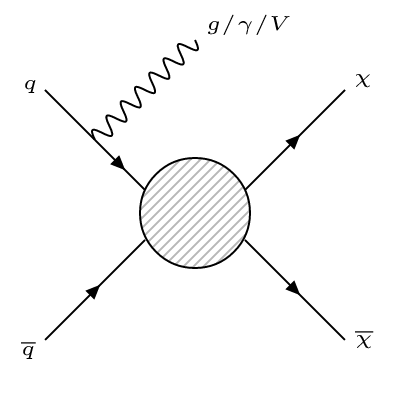
\includegraphics[width=2in]{figures/isr.png}
\caption{}
\label{fig:isr}
\end{subfigure}
\begin{subfigure}{0.45\textwidth}
\centering
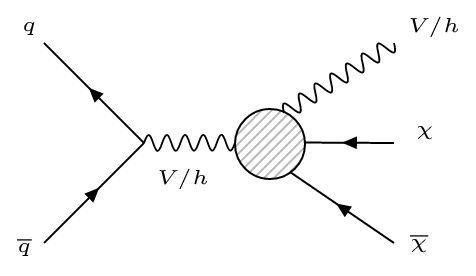
\includegraphics[width=2.5in]{figures/fsr.png}
\caption{}
\label{fig:fsr}
\end{subfigure}
\caption{(a) Mono-X production topology for signatures with X emitted as ISR. (b) Mono-X production topology for signatures with X emitted from new physics vertex.}
\label{monox}
\end{figure}

Mono-H searches have been done at the 8 TeV LHC for H decaying to two photons \cite{Aad:2015yga} and two b quarks \cite{Aad:2015dva} at ATLAS, with results consistent with SM predictions and limits set on various model parameters. The bb final state shows a higher sensitivity to limit setting for the models used in the data interpretation at 8 TeV. For 13 TeV LHC data, mono-H searches are being done at ATLAS for H to bb \cite{Atlas:2016Hbb} and at CMS for the five H decay modes: ZZ, WW \cite{CMS-AN-15-338}, $\gamma\gamma$ \cite{CMS-AN-15-203}, bb \cite{CMS-AN-15-209}, and $\tau\tau$ \cite{CMS-AN-15-???}. Each final state will have various benefits and drawbacks, with a distinct analysis dedicated to each, exploring the sensitivity to different models in different regions of parameter space.

The H$\rightarrow$ZZ decay mode is studied in this dissertation, where the two Z bosons decay to four leptons. The mode where the Z bosons decay to two leptons and two neutrinos is open for investigation. The four lepton final state has the advantage over other H decay modes of easily reducible backgrounds and a clean reconstruction of final state particles. The three lepton combinations of four electrons, four muons, and two electrons two muons are treated individually, then combined in the final results. This channel was key to the discovery of H \cite{Chatrchyan:2013mxa, ATLAS:2013nma} at 7 and 8 TeV, and this analysis is an extension of these studies and their continuation \cite{CMS-AN-15-277, CMS-PAS-HIG-15-004}. In particular, the baseline event selection used here and detailed below is chosen to match that of the other H$\rightarrow$ZZ analysis groups through an event by event synchronization exercise \cite{synchtwiki}.

Nine kinematically distinct models with DM are used in the data interpretation, including five effective field theory (EFT) models and four simplified models. The EFT models couple DM to H via an n-dimensional contact operator, with operators of dimension four, five, six, and eight \cite{Carpenter:2013xra}. They have the benefit of being independent of the details of new physics models and having a one-dimensional parameter space. The EFTs have the drawback of limited ranges of validity, being constrained by perturbativity and H and Z to invisible decay limits. The EFT parameter choices are discussed in the next section. The simplified models introduce an additional massive particle to mediate the DM-SM coupling. This mediator particle is a vector, scalar, or pseudoscalar \cite{Carpenter:2013xra, Berlin:2014cfa}. Although they are better motivated by the addition of new physics, the simplified models have the drawback of more complex parameter spaces, including parameters which affect the kinematics of the final state particles and must be scanned over. The simplified model parameter choices are discussed in the next section, and are chosen to be consistent with other LHC DM searches \cite{Abercrombie:2015wmb}.

\subsection{Signal Models}

The signal models are divided into two categories: effective field theories (EFTs) and simplified models.

\subsubsection{Effective Field Theory Models and Benchmarks}

The five EFTs are summarized in Table~\ref{tab:efts}. The models have Lagrangians with effective operators ranging from dimension four to eight with either scalar or fermionic DM \cite{McDonald:1993ex, LopezHonorez:2012kv}, producing mono-H signatures shown in Figure~\ref{fig:eftsig}. The models have two parameters each, the DM mass and the coupling or mass cutoff scale. In general, the kinematics depend on the choice of both parameters, although there are regions of parameter space where the kinematics are independent of the coupling or mass cutoff scale. The DM mass values are the same for all models, 
\begin{center}
1, 10, 50, 65, 100, 200, 400, 800, 1000, 1300 GeV
\end{center}
as recommended by the DMWG in \cite{Abercrombie:2015wmb}. These mass values are chosen with a fine enough grid spacing to cover the range of variation in kinematics. The additional value of 65 GeV, around half the Higgs mass, is added where the cross sections begin to drop significantly and assists in producing smooth limit curves.

\begin{figure}[tbh]
\centering
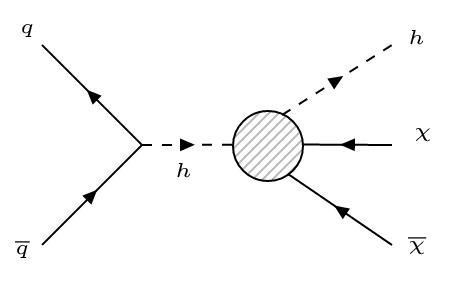
\includegraphics[width=3in]{figures/eftsig.png}
\caption{Collider production diagram for mono-H EFTs.}
\label{fig:eftsig}
\end{figure}

The value of the coupling must be set for each model individually so as to ensure the value is in a range where the kinematics are independent of the coupling. In these regions of parameter space, cross section limits can be reliably scaled to coupling limits. The additional value of $\Lambda = 1000 GeV$ for EFT$\_$xdxHDHc is included to compare with Run 1 limits even though it is in the region where the kinematics depend on the coupling. Existing constraints on the couplings from perturbativity \cite{Carpenter:2013xra} and invisible branching ratio limits \cite{Belanger:2013kya, PhysRevD.86.010001} are shown in Table~\ref{tab:eftlims}. The constraints from invisible branching ratio limits only apply when the DM mass is less than half the mediator mass, allowing this decay to be kinematically open. The production cross sections for these benchmark choices are given in Appendix A.

\begin{table*}[htbH]
\begin{center}
\begin{tabular}{ l | c | l | c | c}
\hline
Name & Operator & Param. & Dim. & $S_{\chi}$ \\
\hline
EFT$\_$HHxx$\_$scalar & $\lambda |H|^{2} \chi^{2}$ & $m_{\chi}, \lambda = 0.1$ & 4 & 0 \\
EFT$\_$HHxx$\_$combined & $\frac{1}{\Lambda} |H|^{2} \bar{\chi} \chi$ & $m_{\chi}, \Lambda = 1000$ GeV & 5 & 1/2 \\
EFT$\_$HHxxg5x & $\frac{1}{\Lambda} |H|^{2} \bar{\chi} i \gamma_{5} \chi$ & $m_{\chi}, \Lambda = 100$ GeV & 5 & 1/2\\
EFT$\_$xdxHDHc & $\frac{1}{\Lambda^{2}} \chi^{\dag} i \partial^{\mu} \chi H^{\dag} i D_{\mu} H $ & $m_{\chi}, \Lambda = 100,1000$ GeV & 6 & 0\\
EFT$\_$xgxFHDH & $\frac{1}{\Lambda^{4}} \bar{\chi} \gamma^{\mu} \chi B_{\mu\nu} H^{\dag} D^{\nu} H$ & $m_{\chi}, \Lambda = 200$ GeV & 8 & 1/2\\
\hline
\end{tabular}
\caption{Effective Field Theory Models.}\label{tab:efts}
\end{center}
\end{table*}

\begin{table*}[htbH]
\begin{center}
\begin{tabular}{ l | c | l}
\hline
Name & Perturbativity & $BR_{inv}$ Limits \\
\hline
EFT$\_$HHxx$\_$scalar & $\lambda < 4\pi$ & $\lambda < 0.016$ ($m_\chi < m_h/2$)\\
EFT$\_$HHxx$\_$combined & $\Lambda > v/4\pi $ & $\Lambda > 10$ TeV ($m_\chi < m_h/2$)\\
EFT$\_$HHxxg5x & $\Lambda > v/4\pi $ & $\Lambda > 10$ TeV ($m_\chi < m_h/2$) \\
EFT$\_$xdxHDHc & $g_Z < 4\pi$, $\Lambda > 30$ GeV & $\Lambda > 400$ GeV ($m_\chi < m_Z/2$) \\
\hline
\end{tabular}
\caption{Constraints on EFT parameters.}\label{tab:eftlims}
\end{center}
\end{table*}

\subsubsection{Simplified Models}

\indent There are four simplified models, each including one or more new massive particles that mediate the H-DM interaction. The models with vector mediators are motivated by the addition of new symmetries to the Standard Model, with the mediator corresponding to the gauge boson of the new symmetry. Additional models are motivated by the addition of scalar or pseudoscalar mediators as a portal into the dark sector.

\subsubsection{Z' - Two Higgs Doublet Model}

The Z' - Two Higgs Doublet Model (Zp2HDM) simplified model extends the gauge group of the SM in include a new symmetry, $U(1)_{Z'}$, with Z' the gauge boson \cite{Berlin:2014cfa}. This symmetry is spontaneously broken by a scalar singlet $\phi$, generating a Z' mass above the EW symmetry breaking scale. The right-handed quarks are charged under $U(1)_{Z'}$ and all other SM particles are neutral. The Z' coupling to quarks, $g_z$, is constrained by EW global fits \cite{PhysRevD.86.010001} and dijet resonance searches \cite{Aaltonen:2008dn, Chatrchyan:2013qha} to be

\begin{equation}
g_z < 0.03 \frac{g}{\cos\theta_w\sin^2\beta}\frac{\sqrt{M_{Z'}^2-M_Z^2}}{M_Z}.
\end{equation}

Additionally, a second Higgs doublet is added with a Type 2 two-Higgs doublet model, introducing states $\Phi_u$ and $\Phi_d$, which couple to up and down type quarks respectively as

\begin{equation}
\mathcal{L} \supset -y_u Q \bar{\Phi}_u \bar{u} - y_d Q \Phi_d \bar{d} + y_e L \Phi_d \bar{e} + h.c..
\end{equation}

$\Phi_u$ is chosen to be charged under $U(1)_{Z'}$, while $\Phi_d$ is neutral. The two Higgs doublets obtain vevs $\nu_u$ and $\nu_d$ after EW symmetry breaking and can be parametrized as

\begin{equation}
\begin{split}
\Phi_d = \frac{1}{\sqrt{2}} \begin{pmatrix}-\sin(\beta) H^{+} \\ \nu_d - \sin(\alpha)h + \cos(\alpha)H - i\sin(\beta)A^0 \end{pmatrix} \\
\Phi_u = \frac{1}{\sqrt{2}} \begin{pmatrix} \cos(\beta)H^{+} \\  \nu_u + \cos(\alpha)h + \sin(\alpha)H + i\cos(\beta)A^0 \end{pmatrix}
\end{split}
\end{equation}

where $h$ and $H$ are neutral CP-even scalars and $A^0$ is CP-odd. The angle $\alpha$ is defined as the angle that diagonalizes the $h-H$ mass mixing matrix, and the angle $\beta$ is defined as $\tan(\beta) = \nu_u / \nu_d$. $h$ is assumed to be the SM Higgs boson with $m_h = 125$ GeV, while the other scalars have masses $> 300$ GeV. Due to perturbativity and previous constraints \cite{Craig:2013hca}, $\alpha$ and $\beta$ are chosen such that $\tan(\beta)>0.3$ and $\alpha = \beta - \pi/2$.

Mono-Higgs signals arise when the pseudoscalar $A^0$ has a large branching ratio to DM, as shown in Figure~\ref{fig:zp2hdmsig}. The new particles and parameters of the Zp2HDM model are summarized in Table~\ref{tab:Zp2HDM}. The values of the parameters chosen for various benchmark scenarios are given in the next section.

\begin{figure}[tbh]
\centering
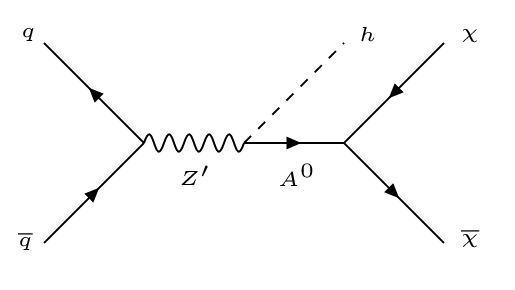
\includegraphics[width=3in]{figures/zp2hdmsig.png}
\caption{Collider production diagram for Zp2HDM.}
\label{fig:zp2hdmsig}
\end{figure}

\begin{table*}[htbH]
\begin{center}
\begin{tabular}{ l | l}
\hline
Particle & Description \\
\hline
$\chi$ & Fermionic DM particle \\
Z' & $U(1)_{Z'}$ gauge boson \\
$\phi$ & Z' sector scalar \\
$\Phi_u, \Phi_d$ & Two Higgs doublets \\
$h, H$ & Neutral CP-even scalars \\
$H^\pm$ & Charged heavy Higgs \\
$A^0$ & Neutral CP-odd pseudoscalar \\
\hline
Param. & Description \\
\hline
$m_\chi$ & DM mass \\
$m_{Z'}$ & Z' mass \\
$g_z$ & Z'-quark coupling \\
$y_{u/d/e}$ & $\Phi$-up-quark/down-quark/lepton coupling \\
$\nu_{u/d}$ & $\Phi_{u/d}$ vev \\
$\alpha$ & $h$-$H$ mixing angle \\
$\beta$ & $\Phi_{u/d}$ vev angle \\
\hline
\end{tabular}
\caption{Zp2HDM simplified model}\label{tab:Zp2HDM}
\end{center}
\end{table*}


\subsubsection{Baryonic Z' Model}

The Baryonic Z' (ZpBaryonic) simplified model extends the gauge group of the SM to include a new symmetry, $U(1)_B$ for the baryon number B, with the Z' being the gauge boson of $U(1)_B$ \cite{Carone:1994aa, Agashe:2004bm, FileviezPerez:2010gw}. Z' couples to quarks and fermionic DM as

\begin{equation}
\mathcal{L} \supset g_q \bar{q} \gamma^\mu q Z'_\mu + g_\chi \bar{\chi} \gamma^\mu \chi Z'_\mu
\end{equation}

To derive a mono-Higgs signature, $U(1)_B$ is spontaneously broken by a "baryonic Higgs" scalar $h_B$, which mixes with the SM Higgs via a mixing angle $\theta$. This mixing induces an h-Z' interaction $-g_{hZ'Z'} h Z'_\mu Z'^\mu$ with coupling

\begin{equation}
g_{hZ'Z'} = \frac{m_{Z'}^2 \sin(\theta)}{\nu_B}
\end{equation}

where $m_{Z'}$ is the mass of the Z' and $\nu_B$ is the vacuum expectation value (vev) of $h_B$. At energies less than $m_{Z'}$, these operators combine to yield an effective Lagrangian

\begin{equation}
\mathcal{L}_{eff} = -\frac{g_q g_\chi}{m_{Z'}^2} \bar{q} \gamma^\mu q \bar{\chi} \gamma_\mu \chi (1 + \frac{g_{hZ'Z'}}{m_{Z'}^2} h)
\end{equation}

The first term gives rise to mono-jet and mono-EW boson signals, while the second yields the mono-Higgs signal shown in Figure~\ref{fig:zpsig}.

\begin{figure}[tbh]
\centering
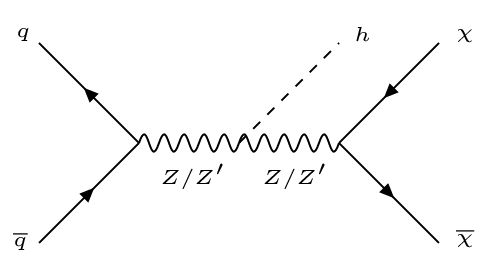
\includegraphics[width=3in]{figures/zpsig.png}
\caption{Collider production diagram for Z' models.}
\label{fig:zpsig}
\end{figure}

The new particles and parameters of the ZpBaryonic model are summarized in Table~\ref{tab:ZpBaryonic}. Perturbativity arguments require the Z'-quark coupling to be less than $4\pi$ \cite{Carpenter:2013xra}. The values of the parameters chosen for various benchmark scenarios are given in the next section.

\begin{table*}[htbH]
\begin{center}
\begin{tabular}{ l | l}
\hline
Particle & Description \\
\hline
$\chi$ & Fermionic DM particle \\
Z' & $U(1)_B$ gauge boson \\
$h_B$ & Baryonic Higgs \\
\hline
Param. & Description \\
\hline
$m_\chi$ & DM mass \\
$m_{Z'}$ & Z' mass \\
$g_q$ & Z'-quark coupling \\
$g_\chi$ & Z'-DM coupling \\
$g_{hZ'Z'}$ & Z'-h coupling \\
$\theta$ & $h$-$h_B$ mixing angle \\
$\nu_B$ & $h_B$ vev \\
\hline
\end{tabular}
\caption{ZpBaryonic simplified model}\label{tab:ZpBaryonic}
\end{center}
\end{table*}

\subsubsection{Hidden Sector Z' Model}

The Hidden Sector Z' (ZpHS) simplified model mixes the SM and a hidden sector with a $U(1)'$ symmetry \cite{Chang:2006fp, Pospelov:2007mp, Feldman:2007wj, Feng:2008mu, Gopalakrishna:2008dv}. SM particles are neutral under $U(1)'$ while DM is charged. The relevant terms in the Lagrangian are

\begin{equation}
\mathcal{L}_{eff} \supset \frac{g_2}{2c_W} J^\mu_{NC} Z_\mu + g_\chi \bar{\chi} \gamma^\mu \chi Z'_\mu
\end{equation}

where $J_{NC}$ is the SM neutral current. A mono-Higgs signature arises from a $Z-Z'$ mass mixing, which is diagonalized by the rotation

\begin{equation}
Z \rightarrow \cos(\theta) Z - \sin(\theta) Z', Z' \rightarrow \cos(\theta) Z' + \sin(\theta) Z
\end{equation}

This mixing yields the mono-Higgs signatures shown in Figure~\ref{fig:zpsig} through the $h-Z-Z'$ interaction 

\begin{equation}
\mathcal{L}_{eff} \supset \frac{m_Z^2 \sin(\theta)}{\nu} h Z'_\mu Z^\mu
\end{equation}

The new particles and parameters of the ZpHS model are summarized in Table~\ref{tab:ZpHS}. In order to be consistent with the invisible $Z$ width of $\Lambda(Z\rightarrow \chi\bar{\chi})<3$ MeV, the value of $\theta$ is constrained by $\sin\theta<0.03$ for $m_\chi < m_z/2$ \cite{PhysRevD.86.010001}. The values of the parameters chosen for various benchmark scenarios are given in the next section.

\begin{table*}[htbH]
\begin{center}
\begin{tabular}{ l | l}
\hline
Particle & Description \\
\hline
$\chi$ & Fermionic DM particle \\
Z' & $U(1)'$ gauge boson \\
\hline
Param. & Description \\
\hline
$m_\chi$ & DM mass \\
$m_{Z'}$ & Z' mass \\
$g_\chi$ & Z'-DM coupling \\
$\theta$ & $Z$-$Z'$ mixing angle \\
\hline
\end{tabular}
\caption{ZpHS simplified model}\label{tab:ZpHS}
\end{center}
\end{table*}

\subsubsection{Scalar Mediator Model}

The Scalar Mediator (Scalar) simplified model introduces a real scalar singlet S as a portal into the dark sector \cite{MarchRussell:2008yu}. The quark and DM Yukawa coupling terms are

\begin{equation}
\mathcal{L} \supset -y_\chi \bar{\chi} \chi S - \frac{m_q}{\nu} \bar{q} q h
\end{equation}

and the relevant terms of the scalar potential are

\begin{equation}
V \supset a |H|^2 + b |H|^2 S^2 + \lambda_h |H|^4 \rightarrow \frac{1}{2} a (h+\nu)^2 S + \frac{1}{2} b (h+\nu)^2 S^2 + \frac{\lambda_h}{4}(h+\nu)^4.
\end{equation}

The expression after the arrow follows when the Higgs acquires a vev, as $H \rightarrow \frac{1}{\sqrt{2}} (h + \nu)$. After expanding the expression, there is an h-S mixing term $a\nu hS$. The system can be diagonalized with the rotation

\begin{equation}
h \rightarrow \cos(\theta) h + \sin(\theta) S, S \rightarrow \cos(\theta) S - \sin(\theta) h
\end{equation}

where $\theta$ is defined by $\sin(2\theta) = 2a\nu/(m_S^2-m_h^2)$. Following this rotation, the Yukawa terms become

\begin{equation}
\mathcal{L} \supset -y_\chi \bar{\chi} \chi (\cos(\theta) S - \sin(\theta) h) - \frac{m_q}{\nu} \bar{q} q (\cos(\theta) h + \sin(\theta) S)
\end{equation}

and the relevant terms in the scalar potential, at first order in $\sin(\theta)$, are

\begin{equation}
V \supset \frac{\sin(\theta)}{\nu}(2m_h^2 + m_S^2) h^2 S + b \nu h S^2.
\end{equation}

These terms give rise to the mono-Higgs interactions shown in Figure~\ref{fig:scsig}, as well as additional loop diagrams for gluon fusion production. The new particles and parameters of the Scalar model are summarized in Table~\ref{tab:Scalar}. Perturbativity arguments require $\sin\theta<4\pi$ \cite{Carpenter:2013xra} while 8 TeV Higgs data is consistent with $\cos\theta=1$, requiring $\sin\theta<0.4$ \cite{Falkowski:2013dza, Djouadi:2013qya, Giardino:2013bma, Ellis:2013lra}. The values of the parameters chosen for various benchmark scenarios are given in the next section.

\begin{figure}[tbh]
\centering
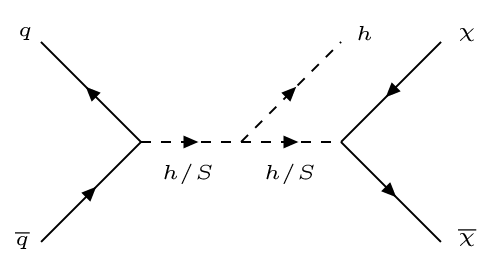
\includegraphics[width=3in]{figures/scsig.png}
\caption{Collider production diagram for Scalar model.}
\label{fig:scsig}
\end{figure}

\begin{table*}[htbH]
\begin{center}
\begin{tabular}{ l | l}
\hline
Particle & Description \\
\hline
$\chi$ & Fermionic DM particle \\
S & Scalar particle \\
\hline
Param. & Description \\
\hline
$m_\chi$ & DM mass \\
$m_{S}$ & S mass \\
$y_\chi$ & S-DM coupling \\
$a, b$ & $h$-$S$ scalar couplings \\
$\theta$ & $h$-$S$ mixing angle \\
\hline
\end{tabular}
\caption{Scalar simplified model}\label{tab:Scalar}
\end{center}
\end{table*}


\subsubsection{Benchmarks}

The simplified models are summarized in Table~\ref{tab:sms}. Although these models have better physical motivations, the parameter spaces are vastly more complex than the EFTs, making it difficult to understand the cross section scaling rules and kinematic dependence on parameters accross the entire parameter spaces. The parameter values are chosen to match the recommendations of the DMWG \cite{Abercrombie:2015wmb}. For the ZpHS (Z' Hidden Sector) model, which is not included in the DMWG report, the coupling parameters are chosen to match the benchmarks in \cite{Carpenter:2013xra} while the DM and mediator mass scan matches the DMWG recommendations for a vector mediator, shown in Table~\ref{tab:MMVector}. The DM and mediator mass scans for the Zp2HDM and Scalar models are shown in Table~\ref{tab:MM2HDM} and Table~\ref{tab:MMScalar}, respectively. Existing constraints on the couplings from theory and invisible branching ratio limits given in \cite{Carpenter:2013xra} are shown in Table~\ref{tab:smlims}. The production cross sections for the simplified models are given in Appendix A. 

\begin{table*}[htbH]
%\begin{center}
%\begin{adjustbox}{width=\textwidth,totalheight=\textheight,keepaspectratio}
\begin{tabular}{ l | c | c | c}
\hline
Name & Mediator($S_{\rm{Mediator}}$) & Fixed Param. & Scanned Param.\\
\hline
Zp2HDM & Z'(1/2) & $m_\chi = 100$ GeV & ($m_{Z'}$,$m_{A^0}$) = Table~\ref{tab:MM2HDM} \\
 & $A^0$(0) & $g_Z = 0.8$ &  \\
 & & $\tan\beta = 1$ &  \\
\hline
ZpBaryonic & Z'(1/2) & $g_\chi = 1$ & ($m_{Z'}$,$m_\chi$) = Table~\ref{tab:MMVector} \\
 & & $g_q = 1/3$ &  \\
 & & $g_{hZ'Z'} = m_{Z'}$ &  \\
\hline
ZpHS & Z'(1/2) & $g_\chi = 1$ & ($m_{Z'}$,$m_\chi$) = Table~\ref{tab:MMVector} \\
 & & $\sin(\theta) = 0.1$ & \\
\hline
Scalar & S(0) & $g_\chi = 1$ & ($m_{S}$,$m_\chi$) = Table~\ref{tab:MMScalar}\\
 & & $\sin(\theta) = 0.3$ & \\
 & & $b = 3$ & \\
\hline
\end{tabular}
\caption{Simplified Models.}\label{tab:sms}
%\end{adjustbox}
%\end{center}
\end{table*}

\begin{table*}[htbH]
\begin{center}
\begin{tabular}{ l | c | c}
\hline
Name & Perturbativity & $BR_{inv}$ Limits \\
\hline
Zp2HDM & & \\
ZpBaryonic & $g_q<4\pi$ & N/A\\
ZpHS & N/A & $\sin(\theta) < 0.03$ ($m_\chi < m_Z/2$) [21] \\
Scalar & $\sin2\theta<4\pi$ & $\sin\theta<0.4$ [6,38-41]\\
\hline
\end{tabular}
\caption{Constraints on simplified model parameters.}\label{tab:smlims}
\end{center}
\end{table*}

\begin{table*}[htbH]
\begin{center}
\begin{tabular}{ l | c | c | c | c | c | c | c | c | c | c}
\hline
$m_\chi$ [GeV] & \multicolumn{10}{|c}{$m_{Z'}$ [GeV]} \\
\hline
1 & 10 & 20 & 50 & 100 & 200 & 300 & 500 & 1000 & 2000 & 10000 \\
10 & 10 & 15 & 50 & 100 & & & & & & 10000 \\
50 & 10 & & 50 & 95  & 200 & 300 & & & & 10000 \\
150 & 10 & & & & 200 & 295 & 500 & 1000 & & 10000 \\
500 & 10 & & & & & & 500 & 995 & 2000 & 10000 \\
1000 & 10 & & & & & & & 1000 & 1995 & 10000 \\
\hline
\end{tabular}
\caption{Mass points for models with a vector mediator.}\label{tab:MMVector}
\end{center}
\end{table*}

\begin{table*}[htbH] 
\begin{center} 
\begin{tabular}{ l | c | c | c | c | c | c | c | c} 
\hline 
$m_{A^0}$ [GeV] & \multicolumn{8}{|c}{$m_{Z'}$ [GeV]} \\ 
\hline 
300 & 600 & 800 & 1000 & 1200 & 1400 & 1700 & 2000 & 2500 \\ 
400 & 600 & 800 & 1000 & 1200 & 1400 & 1700 & 2000 & 2500 \\ 
500 & & 800 & 1000 & 1200 & 1400 & 1700 & 2000 & 2500 \\ 
600 & & 800 & 1000 & 1200 & 1400 & 1700 & 2000 & 2500 \\
700 & & & 1000 & 1200 & 1400 & 1700 & 2000 & 2500 \\ 
800 & & & 1000 & 1200 & 1400 & 1700 & 2000 & 2500 \\ 
\hline
\end{tabular} 
\caption{Mass points for Zp2HDM.}\label{tab:MM2HDM} 
\end{center} 
\end{table*} 

\begin{table*}[htbH] 
\begin{center} 
\begin{tabular}{ l | c | c | c | c | c | c | c | c | c} 
\hline 
$m_\chi$ [GeV] & \multicolumn{9}{c}{$m_{Z'}$ [GeV]} \\ 
\hline 
1 & 10 & 20 & 50 & 100 & 200 & 300 & 500 & 1000 & 10000 \\
10 & 10 & 15 & 50 & 100 & & & & & 10000 \\
50 & 10 & & 50 & 95  & 200 & 300 & & & 10000 \\
150 & 10 & & & & 200 & 295 & 500 & 1000 & 10000 \\
500 & 10 & & & & & & 500 & 995 & 10000 \\
1000 & 10 & & & & & & & 1000 & 10000 \\
\hline
\end{tabular} 
\caption{Mass points for models with a scalar mediator.}\label{tab:MMScalar} 
\end{center} 
\end{table*} 

